\subsection{Preliminaries}
\label{prelim}
This section provides an overview of two concepts that we use in the 
proposed solutions. These include the framework of proof carrying data (PCD) 
and the collective signing (CoSi) protocol.


\subsubsection{Proof Carrying Data (PCD).}
The paradigm of PCD~\cite{chiesa2010proof} allows proving to the correctness of a distributed 
computation involving untrusted parties. It produces a single proof for the output 
that attests not only the correctness of the final result, but also 
the correctness of the entire history of intermediate computations that produced 
this result. Correctness here is defined as a polynomially computable predicate that 
abstracts the properties, or invariants, that must be satisfied.


\begin{figure}[h!]
\centerline{
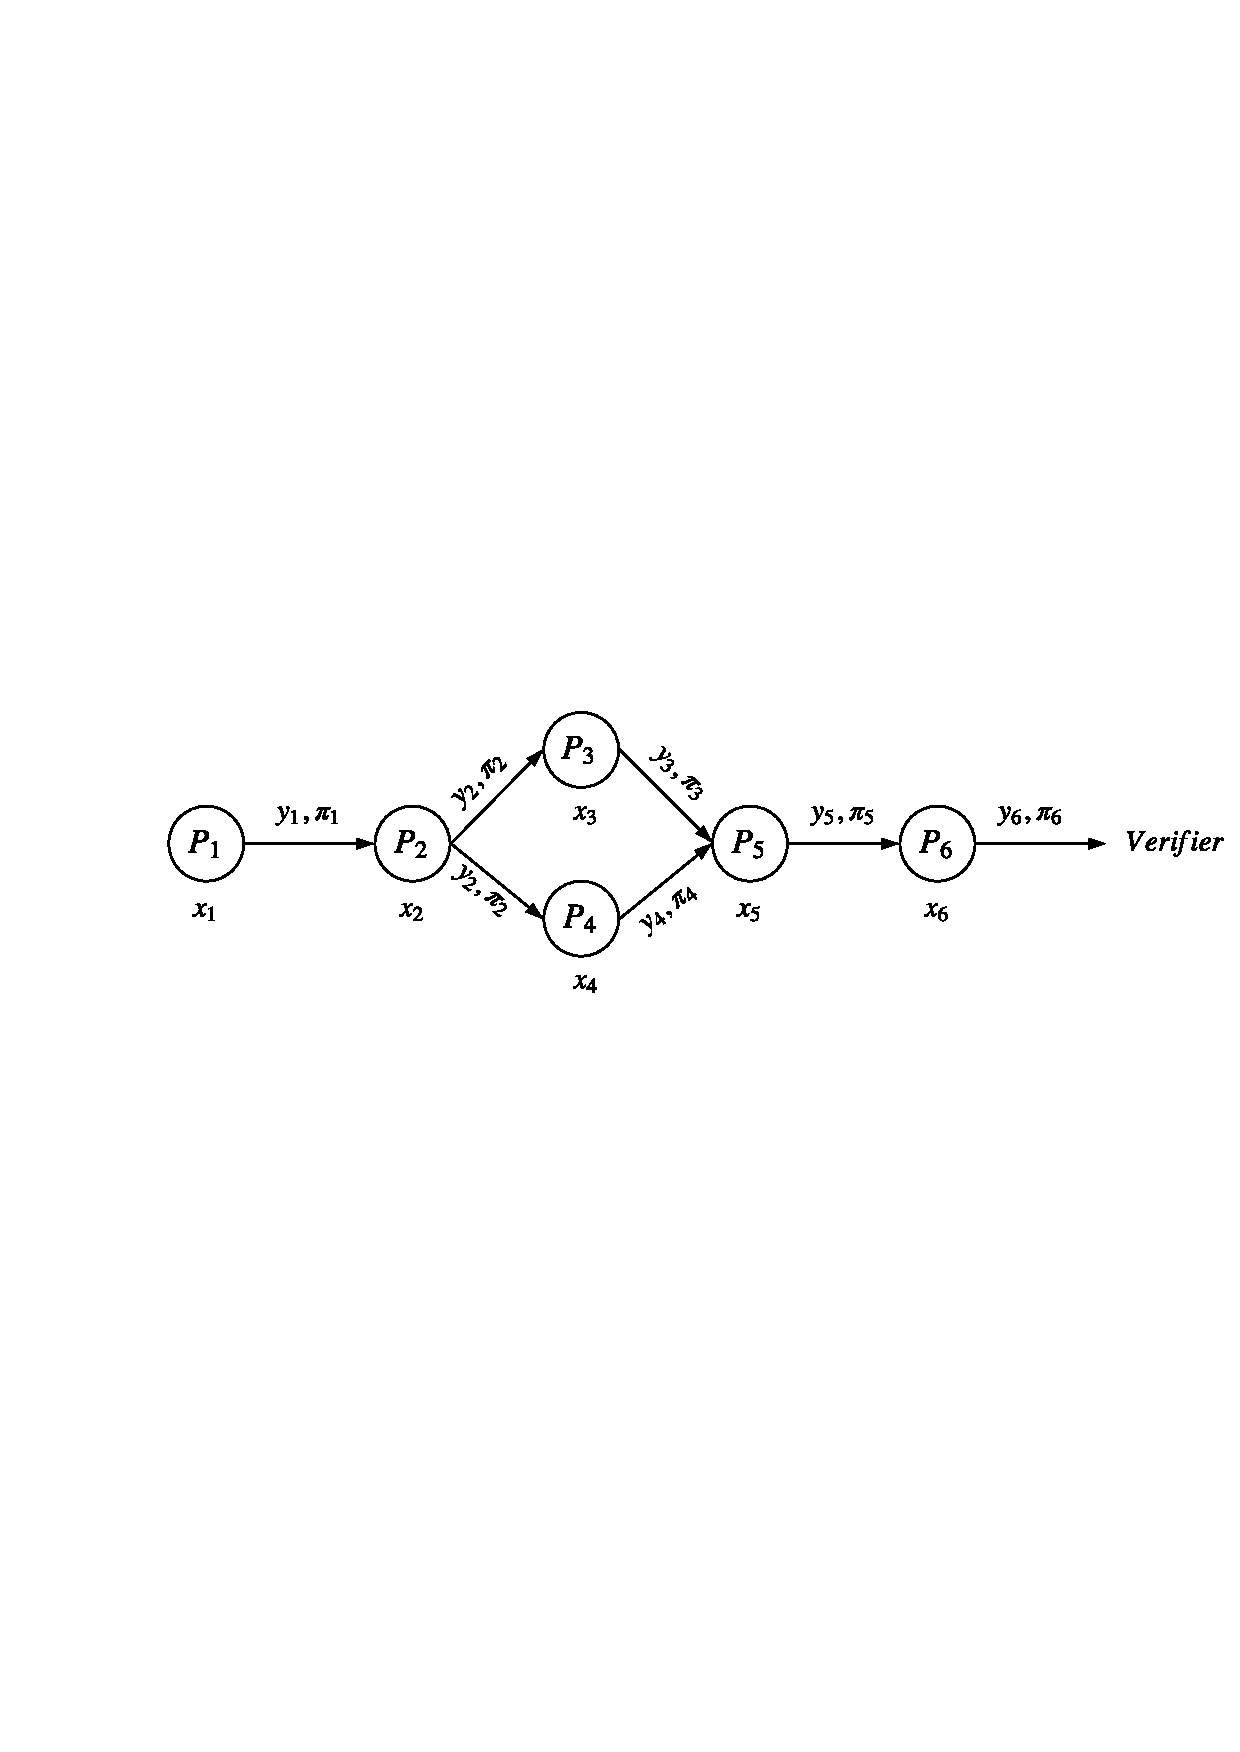
\includegraphics[height= 1.3in, width = 1.0\columnwidth]{figures/pcd-diagram.pdf}}
\caption{An example of a PCD application. A distributed computation involving parties $P_i$, for 
$i \in \{1, \dots, 6\}$, each 
of which has a local input $x_i$ and produces an output $y_i$ with a proof $\pi_i$. }
\label{pcd-diagram}
\end{figure}


To clarify how PDC works, consider a distributed computation task that involves 
the set of parties shown in Figure~\ref{pcd-diagram}. Party $P_1$ starts the computation with its 
own input, produces an intermediate output with a proof saying that it performed 
the computation as defined by the protocol. It then sends both the output and the proof 
to the next party, which is $P_2$ in this case. Here, $P_2$ will 
have its own input $x_2$, as well as everything it received from $P_1$ (including the proof) 
as input to the computation it will perform. Similarly, $P_2$ will produce another 
intermediate output and a proof. This proof not only attests to the correctness of the 
computation done by $P_2$, but also the history that lead to the result $y_2$. In other 
words, it implicitly includes 
the proof from $P_1$. The same process continues until the full computation is finished. 
Anyone can verify the correctness or compliance of the whole distributed protocol by 
only verifying the last proof $\pi_6$ produced by the exit party, which is $P_6$ in the figure.


As shown, PCDs enable untrusted parties to work with each other in a fully distributed 
fashion, without overwhelming the system with the storage and verification of individual 
proofs for each step of the performed protocol. Also, they attest to correctness or compliance  
to the prescribed protocol without re-executing any of the intermediate computations. Thus, 
they provide a promising paradigm for confirming service activity in a compact way.


\subsubsection{Collective Signing (CoSi).}
\label{cosi}
CoSi~\cite{syta2016keeping} is a protocol that enables a set of distributed parties to cosign a 
statement together in a way that produces a single signature. As such, both the 
verification time and the space requirements are just like having a single signer. The 
difference is that this signature attests that all parties agree with the signed 
statement instead of only one.


CoSi builds upon Schnorr 
multisignatures~\cite{schnorr1991efficient, bellare2006multi, micali2001accountable}, but combines 
them with communication trees to speed up the signing process in 
case of a large number of cosigners. In what follows, we only present the protocol
with a plain communication architecture as it suffices for the confirm service activity 
solution introduced in this document.


Schnorr signatures work in a group $\mathbb{G}$ of a prime order $q$ and 
generator $g$, such that the discrete log is believed to be hard in this group. 
Take $n$ parties that want to sign a statement together. 
Each of these parties has a secret $sk_i \in \mathbb{Z}_q$ and a public key 
$pk_i \in \mathbb{G}$ such that $pk_i = g^{sk_i}$. To sign a message $m$, 
one of these parties, let's say $P_1$, coordinates the signing process as follows: 
\begin{enumerate}
\setlength{\itemsep}{0pt}
\item $P_1$ prepares a message $m$ and sends it to the rest of the signers.

\item Each party $P_i$, possibly after verifying 
$m$, selects a secret $\tau_i \in \mathbb{Z}_q$ and compute $V_i = g^{\tau_i}$, 
then it sends $V_i$ back to $P_1$.

\item $P_1$ aggregates all random values received from 
the signers, and its own, by computing $V = \Pi_{i =1}^n V_i$.

\item $P_1$ then computes 
$c = H(V||m)$, where $H$ is an appropriate hash function. $P_1$ then 
sends $c$ to the rest of the parties.

\item Each party computes a response $r_i = \tau_i - sk_i\cdot c$ and 
sends it to $P_1$.

\item Lastly, $P_1$ computes $r = \sum_{i=1}^n r_i$, and outputs the 
collective signature over $m$ as $(c, r)$.
\end{enumerate}


Verifying the signature proceeds as in classical Schnorr signatures~\cite{schnorr1991efficient} with 
one difference. An aggregated public key $pk$ is used in the verification process, 
which is computed as $pk = \Pi_{i=1}^{n} pk_i$.


The work in~\cite{syta2016keeping} tackles several issues related to 
the availability of the 
signing parties, and optimizing the communication between them. 
We believe that such techniques can be used in the NuCypher network if we adopt the 
CoSi-based solution for the confirm service activity issue.

